\documentclass[numbers=noenddot,12pt,a4paper]{scrartcl}
\usepackage[greek,ngerman]{babel}
\usepackage[T1]{fontenc}
\usepackage[utf8]{inputenc}
\usepackage{fullpage}
\usepackage{libertine}
\usepackage{ziffer}
\usepackage{graphicx}
\usepackage{units}
\usepackage[infoshow]{tabularx}
\usepackage{amsmath}
\usepackage{amssymb}
\usepackage{wrapfig}
\usepackage{esint}
\usepackage{float}
\usepackage{wrapfig}
\usepackage[font=small]{caption}
\usepackage{subcaption}
\usepackage{lscape}
\usepackage{hyperref}

\renewcommand{\thefigure}{Abb. \arabic{figure}}

\captionsetup[wrapfigure]{name=}
\captionsetup[figure]{name=}
\newcommand{\degree}{^\circ}
\newcommand{\diff}{\textnormal{d}}
\newcommand{\tenpo}[1]{\cdot 10^{#1}}
\newcommand{\greek}[1]{\greektext#1\latintext}
\newcommand{\ix}[1]{_\text{#1}}
\newcommand{\imag}{\mathbf{i}}

\title{Protokoll: Solarzelle}
\author{Tom Kranz, Philipp Hacker}
\date{\today}

\begin{document}
%\setcounter{page}{2}
%\setcounter{section}{1}
\maketitle
\begin{center}
Betreuer: J. Walowski\\
Versuchsdatum: 4.11.2014/5.11.2014\\
\begin{table}[h]
\centering
Note: %TODO Gute Note erhalten :)
\begin{tabularx}{1.5cm}{|X|}
\hline \\ \\
\hline
\end{tabularx}
\end{table}
\end{center}
\vspace*{\fill}
\tableofcontents
\vfill
\newpage
\section{Einleitung}
Solarzellen sind aktive elektrische Bauelemente zur Umwandlung von Strahlungs- in elektrische Energie. In diesem Versuch sollen die Eigenschaften einer Solarzelle im Betrieb beleuchtet werden -- dazu wird die Strom- und Spannungs-Charakteristik einer handelsüblichen Solarzelle unter verschiedenen Bedingungen aufgenommen und näher ausgewertet. Insbesondere wird dabei auf den Diodencharakter dieses Halbleiterbauelements eingegangen.
\section{Grundlegendes}
Die einfache Solarzelle ist ein Halbleiterbauelement, genauer gesagt: Eine Diode. Als solche benötigt das Verständnis ihrer Funktionsweise Kenntnis von den Eigenschaften von Halbleitern und besonders von p-n-Übergängen.
\subsection{Halbleiter}
\begin{wrapfigure}{r}{0.4\textwidth}
	\vspace{-3em}
	\includegraphics[width=0.4\textwidth]{ebmde.pdf}
	\caption{Schema der Energiebänder in verschiedenen Materialklassen}
	\label{img:Eniv}
\end{wrapfigure}
Halbleiter sind Stoffe, deren elektrische Leitfähigkeit je nach Anwendungsgebiet mehr oder weniger leicht um Größenordnungen verändert werden kann, zum Beispiel durch Veränderung der Temperatur. Diese Eigenschaft verdanken Halbleitermaterialen ihrem besonderen atomaren Aufbau: Die Bindung der sie ausmachenden Teilchen erfolgt durch die einzigen vier Valenzelektronen dieser Teilchen. Praktisch heißt das, dass es am absoluten Nullpunkt keine freien Ladungsträger im Material gibt, da alle Elektronen entweder zu stark an die Atomrümpfe oder in den Bindungen zu den Nachbarteilchen gebunden sind. Wird dem Material Energie zugeführt, können die Elektronen diese in gewissen Maßen quasi ohne Quantelung aufnehmen, da das Potential, in dem diese Quantenobjekte leben, aufgrund der vielen umgebenden Elektronen (und Atomrümpfe) dicht beieinanderliegende, in guter Näherung kontinuierliche, Energieniveaus zulässt. Diese Tatsache wird im sogenannten Bändermodell berücksichtigt. Demnach können sich die Elektronenenergien in kontinuierlichen, aber voneinander unterscheidbarern, Energiebändern bewegen. Bei Halbleitern ist das bei einer bestimmten Temperatur besetzte Valenzband von dem darauffolgenden, höherenergetischen Leitungsband durch eine Bandlücke getrennt -- in diesem Energiebereich gibt es für die Elektronen keine Zustände; entweder die zugeführten Energiequanten reichen zum Überwinden die Bandlücke und Elektronen können ins höhergelegene Band gelangen oder sie nehmen keine Energie auf und verbleiben im Valenzband. Der "`Unterschied"' zu Isolatoren besteht darin, dass es mit angemessenem technischen Aufwand möglich ist, ausreichend vielen Elektronen die Überwindung der Bandlücke zu ermöglichen (vgl. \ref{img:Eniv}, "`Eigenhalbleiter"').
\subsection{p-n-Übergang}

\section{Auswertung}
\begin{figure}[H]
	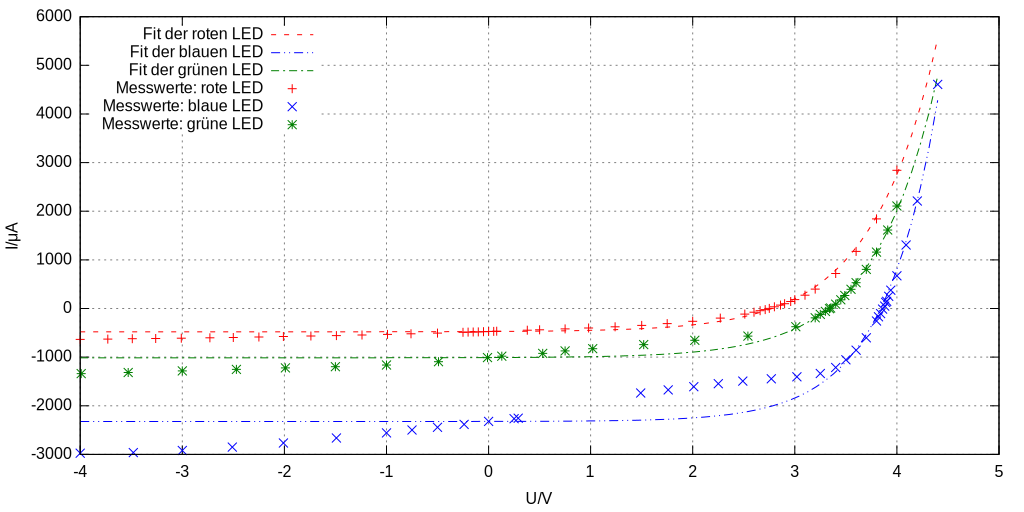
\includegraphics[width=1\textwidth]{messwerte/stromspannungspannungsrichtigled.pdf}
	\caption{Diagramm: Beleuchtung mit LEDs} \label{img:ssrl}
\end{figure}
\begin{figure}[H]
	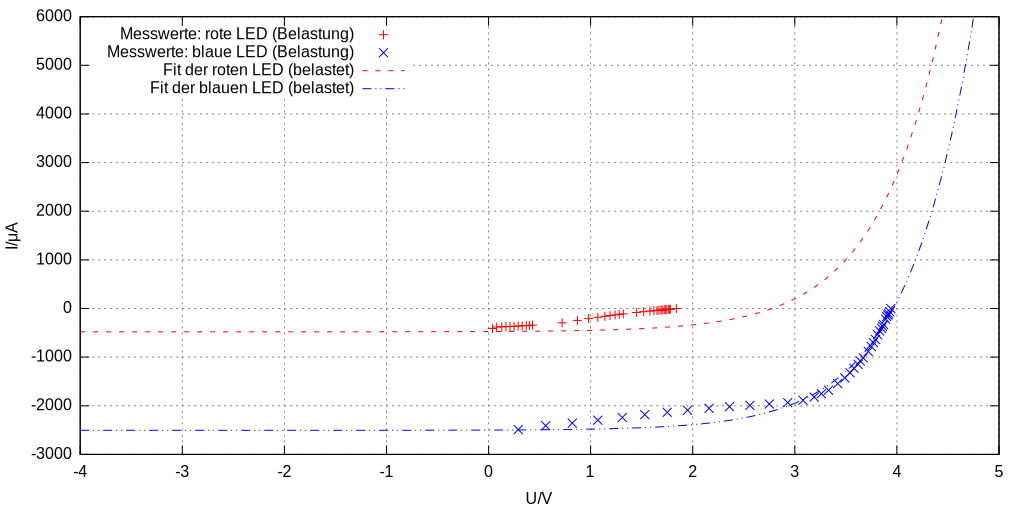
\includegraphics[width=1\textwidth]{messwerte/stromspannungspannungsrichtigbelastungled.pdf}
	\caption{Diagramm: LEDs unter Belastung} \label{img:ssrbl}
\end{figure}
\begin{figure}[H]
	\includegraphics[width=1\textwidth]{messwerte/stromspannunglampeundsonne.pdf}
	\caption{Diagramm: Sonne und Lampe} \label{img:sslus}
\end{figure}
\begin{table}[H]
	\begin{align*}
	\begin{array}{c|c|c|c|c}
		\text{Bedingungen} & \unit[I\ix{S}]{/\text{\greek{μ}}A} & \unit[U\ix{T}^{-1}]{/V}  & \unit[I\ix{F}]{/\text{\greek{µ}}A} & \unit[U\ix{L}]{/V} \\ \hline
		\text{rote LED} & 6,281956078909 & 1,56064714637827 & 473,0 & 2,77744246007079 \\
		\text{blaue LED} & 1,77003245210862 & 1,86925090897572 & 2322,0 & 3,8410832084248 \\
		\text{grüne LED} &  4,54448863386492 & 1,62510156480855 & 1009,0 & 3,32735735941798 \\
		\text{rot; belastet} & 10814,3718863988 & 0,0219641096968227 & 440,0 & 1,81572056047675 \\
		\text{blau; belastet} & 5,22143450482523 & 1,55627173168713 & 2500,0 & 3,96676242807082 \\
		\text{Lampe} &  0,0126470767138272 & 1,96820510727951 & 54,1 & 4,24823463781785 \\
		\text{Lampe; belastet} & 0,000485193181770913 & 2,71513840381794 & 66,0 & 4,35359962136445 \\
		\text{Sonne; belastet} & 6,1828673863364\tenpo{-5} & 2,649501319308 & 15,0 & 4,67982316346892 \\
	\end{array}
	\end{align*}
	\caption{Fitparameter der unter \ref{img:ssrl} bis \ref{img:sslus} gezeigten Graphen} \label{tab:fits}
\end{table}

\section{Anhang}
\subsection{Messwerte}
\begin{table}[H]
	\begin{align*}
\begin{array}{c|c}
\unit[U]{/V} & \unit[I]{/\text{\greek{µ}}A}\\\hline
	-4,00 & -636 \\
	-3,73 & -629 \\
	-3,49 & -622 \\
	-3,26 & -617 \\
	-3,01 & -610 \\
	-2,73 & -602 \\
	-2,50 & -596 \\
	-2,25 & -586 \\
	-2,01 & -576 \\
	-1,74 & -566 \\
	-1,49 & -557 \\
	-1,24 & -545 \\
	\end{array}
	\hspace{2em}
	\begin{array}{c|c}
	\unit[U]{/V} & \unit[I]{/\text{\greek{µ}}A}\\\hline
	-0,99 & -533 \\
	-0,76 & -521 \\
	-0,50 & -506 \\
	-0,25 & -490 \\
	-0,20 & -486 \\
	-0,15 & -484 \\
	-0,10 & -481 \\
	-0,05 & -478 \\
	0,00 & -473 \\
	0,05 & -470 \\
	0,08 & -467 \\
	0,38 & -446 \\
	\end{array}
	\hspace{2em}
	\begin{array}{c|c}
	\unit[U]{/V} & \unit[I]{/\text{\greek{µ}}A}\\\hline
	0,50 & -438 \\
	0,75 & -420 \\
	0,98 & -401 \\
	1,24 & -377 \\
	1,50 & -347 \\
	1,75 & -311 \\
	2,00 & -263 \\
	2,27 & -198 \\
	2,51 & -116 \\
	2,60 & -77 \\
	2,66 & -46 \\
	2,71 & -22 \\
	\end{array}
	\hspace{2em}
	\begin{array}{c|c}
	\unit[U]{/V} & \unit[I]{/\text{\greek{µ}}A}\\\hline
	2,75 & 2 \\
	2,80 & 34 \\
	2,86 & 70 \\
	2,90 & 99 \\
	2,96 & 143 \\
	3,00 & 182 \\
	3,10 & 273 \\
	3,20 & 398 \\
	3,40 & 719 \\
	3,60 & 1175 \\
	3,80 & 1843 \\
	4,00 & 2842
\end{array}  
\end{align*}
\vspace{-1em}
\caption{Messwerte bei Beleuchtung mit der roten LED}
\end{table}


\begin{table}[H]
	\begin{align*}
	\begin{array}{c|c|c}
	\unit[U]{/V} & \unit[I]{/\text{\greek{µ}}A} & \unit[R]{/k\text{\greek{Ω}}}\\\hline
	0,04 & -412 & 0 \\
	0,08 & -380 & 0,1 \\
	0,13 & -376 & 0,2 \\
	0,17 & -373 & 0,3 \\
	0,21 & -370 & 0,4 \\
	0,25 & -366 & 0,5 \\
	0,29 & -360 & 0,6 \\
	0,33 & -356 & 0,7 \\
	0,37 & -351 & 0,8 \\
	0,40 & -347 & 0,9 \\
	0,43 & -341 & 1, \\
	0,72 & -294 & 2, \\
	\end{array}
	\hspace{2em}
	\begin{array}{c|c|c}
	\unit[U]{/V} & \unit[I]{/\text{\greek{µ}}A} & \unit[R]{/k\text{\greek{Ω}}}\\\hline
	0,87 & -244 & 3, \\
	0,98 & -207 & 4, \\
	1,07 & -180 & 5, \\
	1,14 & -160 & 6, \\
	1,19 & -145 & 7, \\
	1,24 & -132 & 8, \\
	1,28 & -121 & 9, \\
	1,32 & -112 & 10, \\
	1,45 & -82,4 & 15, \\
	1,52 & -65,3 & 20, \\
	1,58 & -54,2 & 25, \\
	1,62 & -46,2 & 30, \\
	\end{array}
	\hspace{2em}
	\begin{array}{c|c|c}
	\unit[U]{/V} & \unit[I]{/\text{\greek{µ}}A} & \unit[R]{/k\text{\greek{Ω}}}\\\hline
	1,65 & -40,4 & 35, \\
	1,67 & -35,8 & 40, \\
	1,69 & -32,2 & 45 \\
	1,70 & -29,2 & 50, \\
	1,72 & -26,8 & 55, \\
	1,73 & -24,6 & 60, \\
	1,74 & -21,3 & 70, \\
	1,76 & -18,8 & 80, \\
	1,77 & -16,8 & 90, \\
	1,78 & -15,2 & 100, \\
	1,84 & 0,00 & \approx\infty \\		
	\, & \, & \,
	\end{array}  
	\end{align*}
	\vspace{-1em}
	\caption{Messwerte bei Beleuchtung mit der roten LED unter angegebener Belastung}
\end{table}
\begin{table}[H]
	\begin{align*}
	\begin{array}{c|c}
	\unit[U]{/V} & \unit[I]{/\text{\greek{µ}}A}\\\hline
	-4,00 & -2976 \\
	-3,48 & -2962 \\
	-3,00 & -2919 \\
	-2,51 & -2850 \\
	-2,01 & -2766 \\
	-1,49 & -2663 \\
	-1,00 & -2557 \\
	-0,75 & -2498 \\
	-0,50 & -2442 \\
	-0,24 & -2383 \\
	\end{array}
	\hspace{2em}
	\begin{array}{c|c}
	\unit[U]{/V} & \unit[I]{/\text{\greek{µ}}A}\\\hline
	0,00 & -2322 \\
	0,25 & -2266 \\
	0,29 & -2255 \\
	1,49 & -1738 \\
	1,76 & -1673 \\
	2,01 & -1607 \\
	2,25 & -1547 \\
	2,49 & -1492 \\
	2,77 & -1445 \\
	3,02 & -1404 \\
	\end{array}
	\hspace{2em}
	\begin{array}{c|c}
	\unit[U]{/V} & \unit[I]{/\text{\greek{µ}}A}\\\hline
	3,25 & -1337 \\
	3,40 & -1213 \\
	3,50 & -1054 \\
	3,60 & -857 \\
	3,70 & -603 \\
	3,80 & -257 \\
	3,82 & -171 \\
	3,84 & -105 \\
	3,86 & -11,6 \\
	3,88 & 50 \\
	\end{array}
	\hspace{2em}
	\begin{array}{c|c}
	\unit[U]{/V} & \unit[I]{/\text{\greek{µ}}A}\\\hline
	3,89 & 126,3 \\
	3,90 & 149 \\
	3,92 & 250 \\
	3,94 & 377 \\
	4,00 & 672 \\
	4,09 & 1306 \\
	4,20 & 2211 \\
	4,40 & 4608 \\
	\, & \, \\
	\, & \, \\
	\end{array}  
\end{align*}
\vspace{-1em}
\caption{Messwerte bei Beleuchtung mit der blauen LED}
\end{table}

\begin{table}[H]
	\begin{align*}
	\begin{array}{c|c|c}
	\unit[U]{/V} & \unit[I]{/\text{\greek{µ}}A} & \unit[R]{/k\text{\greek{Ω}}}\\\hline
0,29 & -2490 & 0 \\
0,56 & -2410 & 0,1 \\
0,82 & -2356 & 0,2 \\
1,07 & -2297 & 0,3 \\
1,31 & -2242 & 0,4 \\
1,53 & -2181 & 0,5 \\
1,75 & -2134 & 0,6 \\
1,95 & -2091 & 0,7 \\
2,16 & -2053 & 0,8 \\
2,36 & -2020 & 0,9 \\
2,56 & -1992 & 1, \\
2,75 & -1963 & 1,1 \\
2,93 & -1935 & 1,2 \\
\end{array}
\hspace{2em}
\begin{array}{c|c|c}
\unit[U]{/V} & \unit[I]{/\text{\greek{µ}}A} & \unit[R]{/k\text{\greek{Ω}}}\\\hline
3,08 & -1888 & 1,3 \\
3,19 & -1822 & 1,4 \\
3,26 & -1751 & 1,5 \\
3,33 & -1679 & 1,6 \\
3,42 & -1545 & 1,8 \\
3,49 & -1426 & 2, \\
3,54 & -1322 & 2,2 \\
3,58 & -1230 & 2,4 \\
3,62 & -1149 & 2,6 \\
3,64 & -1078 & 2,8 \\
3,67 & -1015 & 3, \\
3,72 & -885 & 3,5 \\
3,75 & -784 & 4, \\
\end{array}
\hspace{2em}
\begin{array}{c|c|c}
\unit[U]{/V} & \unit[I]{/\text{\greek{µ}}A} & \unit[R]{/k\text{\greek{Ω}}}\\\hline
3,77 & -703 & 4,5 \\
3,79 & -637 & 5, \\
3,81 & -536,7 & 6, \\
3,83 & -463,4 & 7, \\
3,85 & -407,7 & 8, \\
3,86 & -363,8 & 9, \\
3,87 & -328,0 & 10, \\
3,89 & -220,9 & 15, \\
3,90 & -166,3 & 20, \\
3,91 & -133,5 & 25, \\
3,92 & -111,4 & 30, \\
3,93 & -67,0 & 50, \\
3,94 & 0,00 & \approx\infty \\
\end{array}
\end{align*}
\vspace{-1em}
\caption{Messwerte bei Beleuchtung mit der blauen LED unter angegebener Belastung}
\end{table}

\begin{table}[H]
	\begin{align*}
	\begin{array}{c|c}
	\unit[U]{/V} & \unit[I]{/\text{\greek{µ}}A}\\\hline
-3,99 & -1338 \\
-3,53 & -1315 \\
-3,00 & -1283 \\
-2,47 & -1252 \\
-1,99 & -1222 \\
-1,50 & -1197 \\
-1,00 & -1162 \\
-0,49 & -1094 \\
\end{array}
\hspace{2em}
\begin{array}{c|c}
\unit[U]{/V} & \unit[I]{/\text{\greek{µ}}A}\\\hline
-0,01 & -1010 \\
0,13 & -980 \\
0,53 & -924 \\
0,75 & -871 \\
1,02 & -827 \\
1,52 & -742 \\
2,02 & -653 \\
2,54 & -568 \\
\end{array}
\hspace{2em}
\begin{array}{c|c}
\unit[U]{/V} & \unit[I]{/\text{\greek{µ}}A}\\\hline
3,01 & -375 \\
3,20 & -192 \\
3,25 & -122 \\
3,30 & -59 \\
3,34 & -4,2 \\
3,35 & 11,3 \\
3,40 & 87,5 \\
3,45 & 179 \\
\end{array}
\hspace{2em}
\begin{array}{c|c}
\unit[U]{/V} & \unit[I]{/\text{\greek{µ}}A}\\\hline
3,49 & 267 \\
3,55 & 394 \\
3,60 & 531 \\
3,70 & 804 \\
3,80 & 1159 \\
3,91 & 1614 \\
4,00 & 2107 \\
\, & \,
	\end{array}  
	\end{align*}
	\vspace{-1em}
	\caption{Messwerte bei Beleuchtung mit der grünen LED}
\end{table}

\begin{table}[H]
	\begin{align*}
	\begin{array}{c|c}
	\unit[U]{/V} & \unit[I]{/mA}\\\hline
	5,00 & 179,8 \\
	4,75 & 100,5 \\
	4,50 & 34,5 \\
	4,27 & -5,71 \\
	0,15 & -53,85 \\
	0,01 & -54,10 \\
	\end{array}
	\hspace{2em}
	\begin{array}{c|c}
	\unit[U]{/V} & \unit[I]{/mA}\\\hline
	-0,25 & -54,38 \\
	-0,51 & -54,66 \\
	-0,75 & -54,93 \\
	-1,00 & -55,34 \\
	-1,26 & -55,85 \\
	-1,50 & -56,00 \\
	\end{array}
	\hspace{2em}
	\begin{array}{c|c}
	\unit[U]{/V} & \unit[I]{/mA}\\\hline
	-1,75 & -56,12 \\
	-2,00 & -56,60 \\
	-2,25 & -57,08 \\
	-2,51 & -57,78 \\
	-2,75 & -58,12 \\
	-3,00 & -58,47 \\
	\end{array}
	\hspace{2em}
	\begin{array}{c|c}
	\unit[U]{/V} & \unit[I]{/mA}\\\hline
	-3,24 & -58,83 \\
	-3,50 & -59,17 \\
	-3,74 & -59,41 \\
	-4,00 & -59,51 \\
	\, & \, \\
	\, & \, \\
	\end{array}  
	\end{align*}
	\vspace{-1em}
	\caption{Messwerte bei Beleuchtung mit der Lampe}
\end{table}
\begin{table}[H]
	\begin{align*}
	\begin{array}{c|c|c}
	\unit[U]{/V} & \unit[I]{/mA} & \unit[R]{/k\text{\greek{Ω}}}\\\hline
	0,165 & 65,7 & 0 \\
	0,93 & 65,4 & 0,01 \\
	1,68 & 64,8 & 0,02 \\
	2,41 & 64,2 & 0,03 \\
	3,10 & 63,1 & 0,04 \\
	3,56 & 58,6 & 0,05 \\
	\end{array}
	\hspace{2em}
	\begin{array}{c|c|c}
	\unit[U]{/V} & \unit[I]{/mA} & \unit[R]{/k\text{\greek{Ω}}}\\\hline
	3,78 & 52,28 & 0,06 \\
	3,91 & 46,52 & 0,07 \\
	3,98 & 41,69 & 0,08 \\
	4,04 & 37,62 & 0,09 \\
	4,08 & 34,34 & 0,1 \\
	4,24 & 18,04 & 0,2 \\
	\end{array}
	\hspace{2em}
	\begin{array}{c|c|c}
	\unit[U]{/V} & \unit[I]{/mA} & \unit[R]{/k\text{\greek{Ω}}}\\\hline
	4,28 & 12,15 & 0,3 \\
	4,30 & 9,20 & 0,4 \\
	4,31 & 7,38 & 0,5 \\
	4,32 & 6,16 & 0,6 \\
	4,33 & 4,63 & 0,8 \\
	4,34 & 0,91 & 4 \\
	\end{array}
	\end{align*}
	\vspace{-1em}
	\caption{Messwerte bei Beleuchtung mit der Lampe unter angegebener Belastung}
\end{table}
\begin{table}[H]
	\begin{align*}
	\begin{array}{c|c|c}
	\unit[U]{/V} & \unit[I]{/\text{\greek{µ}}A} & \unit[R]{/\text{\greek{Ω}}}\\\hline
0,05 & 20,0 & 0 \\
0,063 & 17,0 & 1 \\
0,075 & 15,0 & 2 \\
0,088 & 14,0 & 3 \\
0,098 & 13,2 & 4 \\
0,111 & 12,9 & 5 \\
0,126 & 12,8 & 6 \\
0,147 & 13,3 & 7 \\
0,154 & 12,5 & 8 \\
0,174 & 14,3 & 9 \\
0,185 & 12,5 & 10 \\
0,335 & 12,8 & 20 \\
\end{array}
\hspace{2em}
\begin{array}{c|c|c}
\unit[U]{/V} & \unit[I]{/mA} & \unit[R]{/\text{\greek{Ω}}}\\\hline
0,55 & 14,8 & 30 \\
0,74 & 14,7 & 40 \\
0,90 & 14,0 & 50 \\
0,95 & 13,0 & 60 \\
1,08 & 12,8 & 70 \\
1,25 & 13,1 & 80 \\
1,39 & 12,9 & 90 \\
1,81 & 15,1 & 100 \\
2,68 & 15,1 & 150 \\
3,46 & 14,7 & 200 \\
3,91 & 13,1 & 250 \\
4,12 & 11,63 & 300 \\
\end{array}
\hspace{2em}
\begin{array}{c|c|c}
\unit[U]{/V} & \unit[I]{/mA} & \unit[R]{/\text{\greek{Ω}}}\\\hline
4,27 & 10,32 & 350 \\
4,34 & 9,21 & 400 \\
4,41 & 7,47 & 500 \\
4,46 & 6,32 & 600 \\
4,51 & 5,47 & 700 \\
4,53 & 4,81 & 800 \\
4,56 & 3,87 & 1000 \\
4,62 & 1,96 & 2000 \\
4,65 & 1,31 & 3000 \\
4,66 & 0,78 & 5000 \\
4,67 & 0,394 & 10000 \\
4,68 & 0,198 & 20000 \\
\end{array}
\end{align*}
\vspace{-1em}
\caption{Messwerte "`in der Sonne"' unter angegebener Belastung}
\end{table}
\subsection{Grafiken}
\section{Quellen}
\ref{img:Eniv}: \url{https://de.wikipedia.org/wiki/Datei:Energy_band_model_(DE).svg} (Urheber: Wikipedia-Benutzer Cepheiden)
\end{document}